\section{Signals and Readout}

\subsection{Front-End Readout Electronics}

There are 512 channels per module read out by FSSR2 chips, mounted on a hybrid. The FSSR2 ASIC has been developed at Fermilab for the BTeV experiment \cite{FSSR}. The chip (see Fig.~\ref{fig:fssr2}) features a data-driven architecture (self-triggered, time-stamped). Each of the 128 input channels of the FSSR2 ASIC has a preamplifier, a shaper that can adjust the shaping time (65--125~ns), a baseline restorer (BLR), and a 3-bit ADC. The period of the clock called the beam crossing oscillator (BCO) sets the data acquisition time. The injected charge causes the discriminator on the selected channel to fire, generating a fast trigger output (GOTHIT) followed by readout of the hit data (OUT1) approximately 1.4 $\mu$s after the trigger. The bunch counter clock (BCOCLK) provides the time stamp with which to tag the data. 

\begin{figure}[hbt] 
\centering 
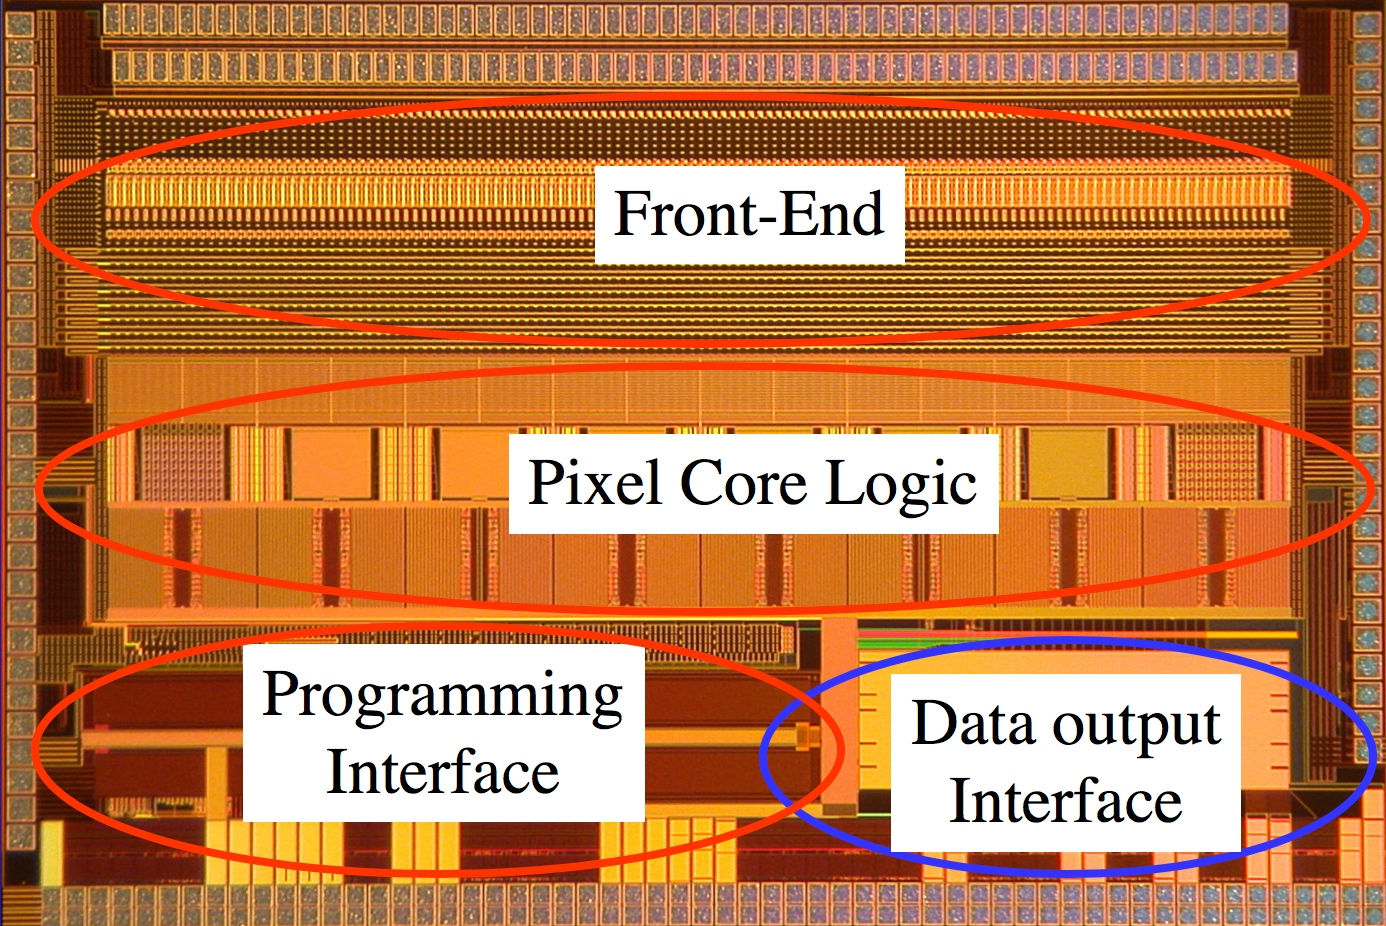
\includegraphics[width=1.0\columnwidth,keepaspectratio]{fssr2.jpg}
\caption{FSSR2 ASIC with the different functional areas labeled.}
\label{fig:fssr2}
\end{figure}

The analog section of the FSSR core consists of 128 channels (see Fig.~\ref{fig:fssr2-analog}). The charge preamplifier integrates the input charge generated in the active volume of the sensor with backplane capacitance C$_D$ and collected through the coupling capacitance C$_{AC}$. The G$_f$ transconductance is used to discharge the feedback capacitance C$_f$. The integrator and shaper are used to improve the signal-to-noise ratio. Its transfer function is CR-(RC)$^2$-type with a programmable peaking time of 65, 85, 100, and 125 ns. The comparator provides the binary information (hit / no hit) to the digital section. The BLR is included to achieve baseline shift suppression. It can be bypassed by a programmable switch. The electronic calibration can be performed either by the internal square-wave pulse generator or by an external pulser, providing voltage steps on the integrated inject capacitance C$_{inj}$ of 40 fF. The injected channels can be selected by a programmable inject mask.  The gain of the preamplifier is also programmable by changing the value of its feedback capacitance \cite{DINARDOTHESIS}.

\begin{figure}[hbt] 
\centering 
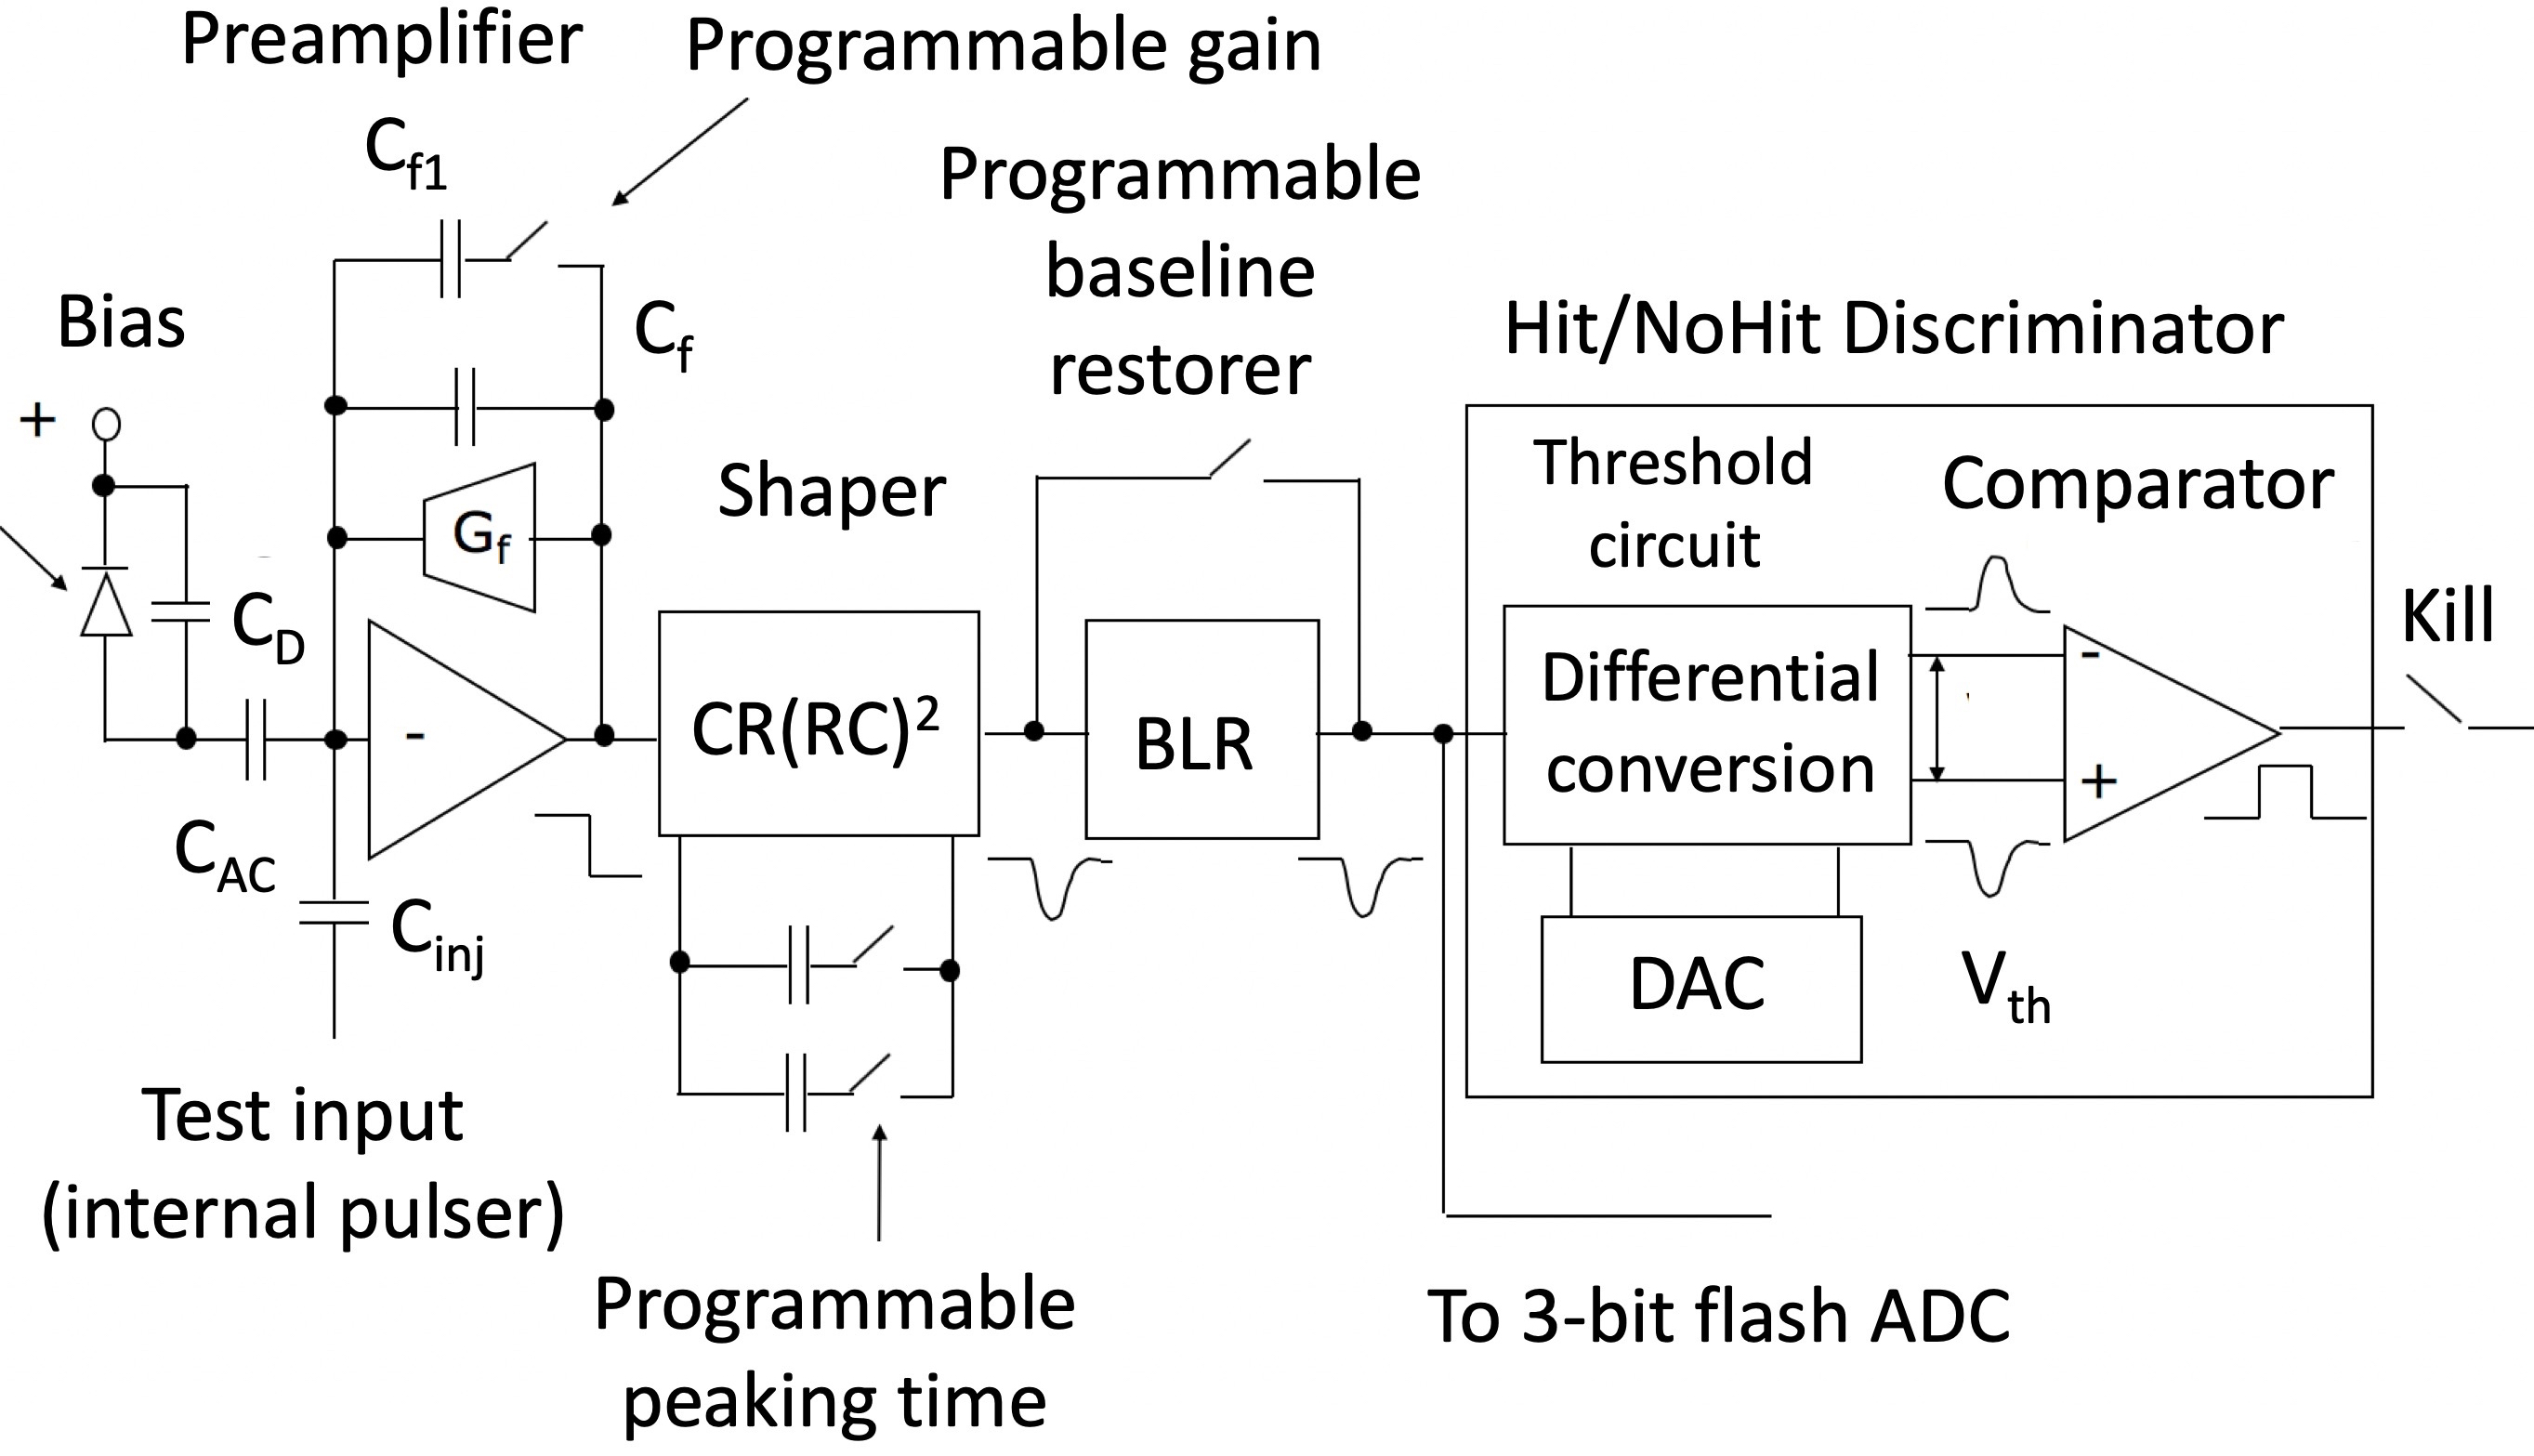
\includegraphics[width=1.0\columnwidth,keepaspectratio]{fssr2-analog.jpg}
\caption{FSSR2 analog channels.}
\label{fig:fssr2-analog}
\end{figure}

If a hit is detected in one of the channels, the core logic transmits pulse amplitude, channel number, and time stamp information to the data output interface. The data output interface accepts data transmitted by the core, serializes it, and transmits it to the data acquisition system. Thus, an irregular data flow is converted into data synchronized with the main clock frequency of the system. No time is allotted for transmitting stored information in the FSSR2 working cycle, i.e., the data arrive at the chip output directly after the signal is detected. The signal reception board should be permanently ready for receiving data, since the data can arrive at any moment. Therefore, the chip can operate only as a part of the software -- hardware complex with the external controller tuned for the data waiting mode (time-variable data flow). 

To send the 24-bit readout words one, two, four, or six LVDS serial data lines can be used. Both edges of the 70~MHz readout clock are used to clock data, resulting in a maximum output data rate of 840 Mb/s. The readout clock is independent of the acquisition clock. Power consumption is $\le$ 4~mW per channel. The FSSR2 is radiation hard up to 5~Mrad. The choice of the readout chip was driven by its architecture and good noise performance at high capacitive load of the long SVT strips.

Each FSSR2 ASICs has six LVDS pairs with a source synchronous clock to transmit event data. The VSCM supports receiving data from all six LVDS pairs of each FSSR2 ASIC running at 70 MHz double data rate (DDR) (840 Mb/s from each FSSR2). Xilinx Spartan 6 FPGAs are used to buffer and deserialize the data from two FSSR2 ASICs each. Four of these FPGAs are used to support eight FSSR2 ASICs' simultaneous data streams coming from two HFCB interfaces; the FPGAs in turn send their information to the master FPGA where the event builder resides.

The FSSR2 ASIC architecture is such that it sends out 24-bit data words if a channel has a hit or a 24-bit status word if the channel does not have a hit (idle state) within a BCO clock cycle. The FSSR2 ASICs transmit these data over six lines. First, the data is de-serialized. The 24-bit data words are appended with 8 bits to make the time range longer, and the 32-bit words are correlated to the trigger, which is generated by other detectors. The status words are suppressed to minimize the data size of an event. However, the status words are monitored to diagnose the performance of individual FSSR2 ASICs. Each channel has a memory cell for writing a single event. If the data on the event arrive into the cell, the channel is disabled, and the data presence signal is sent into the controller. The controller interrogates the channel with the detected event and produces a data word. The data are transmitted in a short time interval, and, after that, the channel is again ready for receiving signals. Under relatively low rates, when the interval between events is longer than the time required for reading a single event, data losses are absent. 

\begin{figure}[hbt] 
\centering 
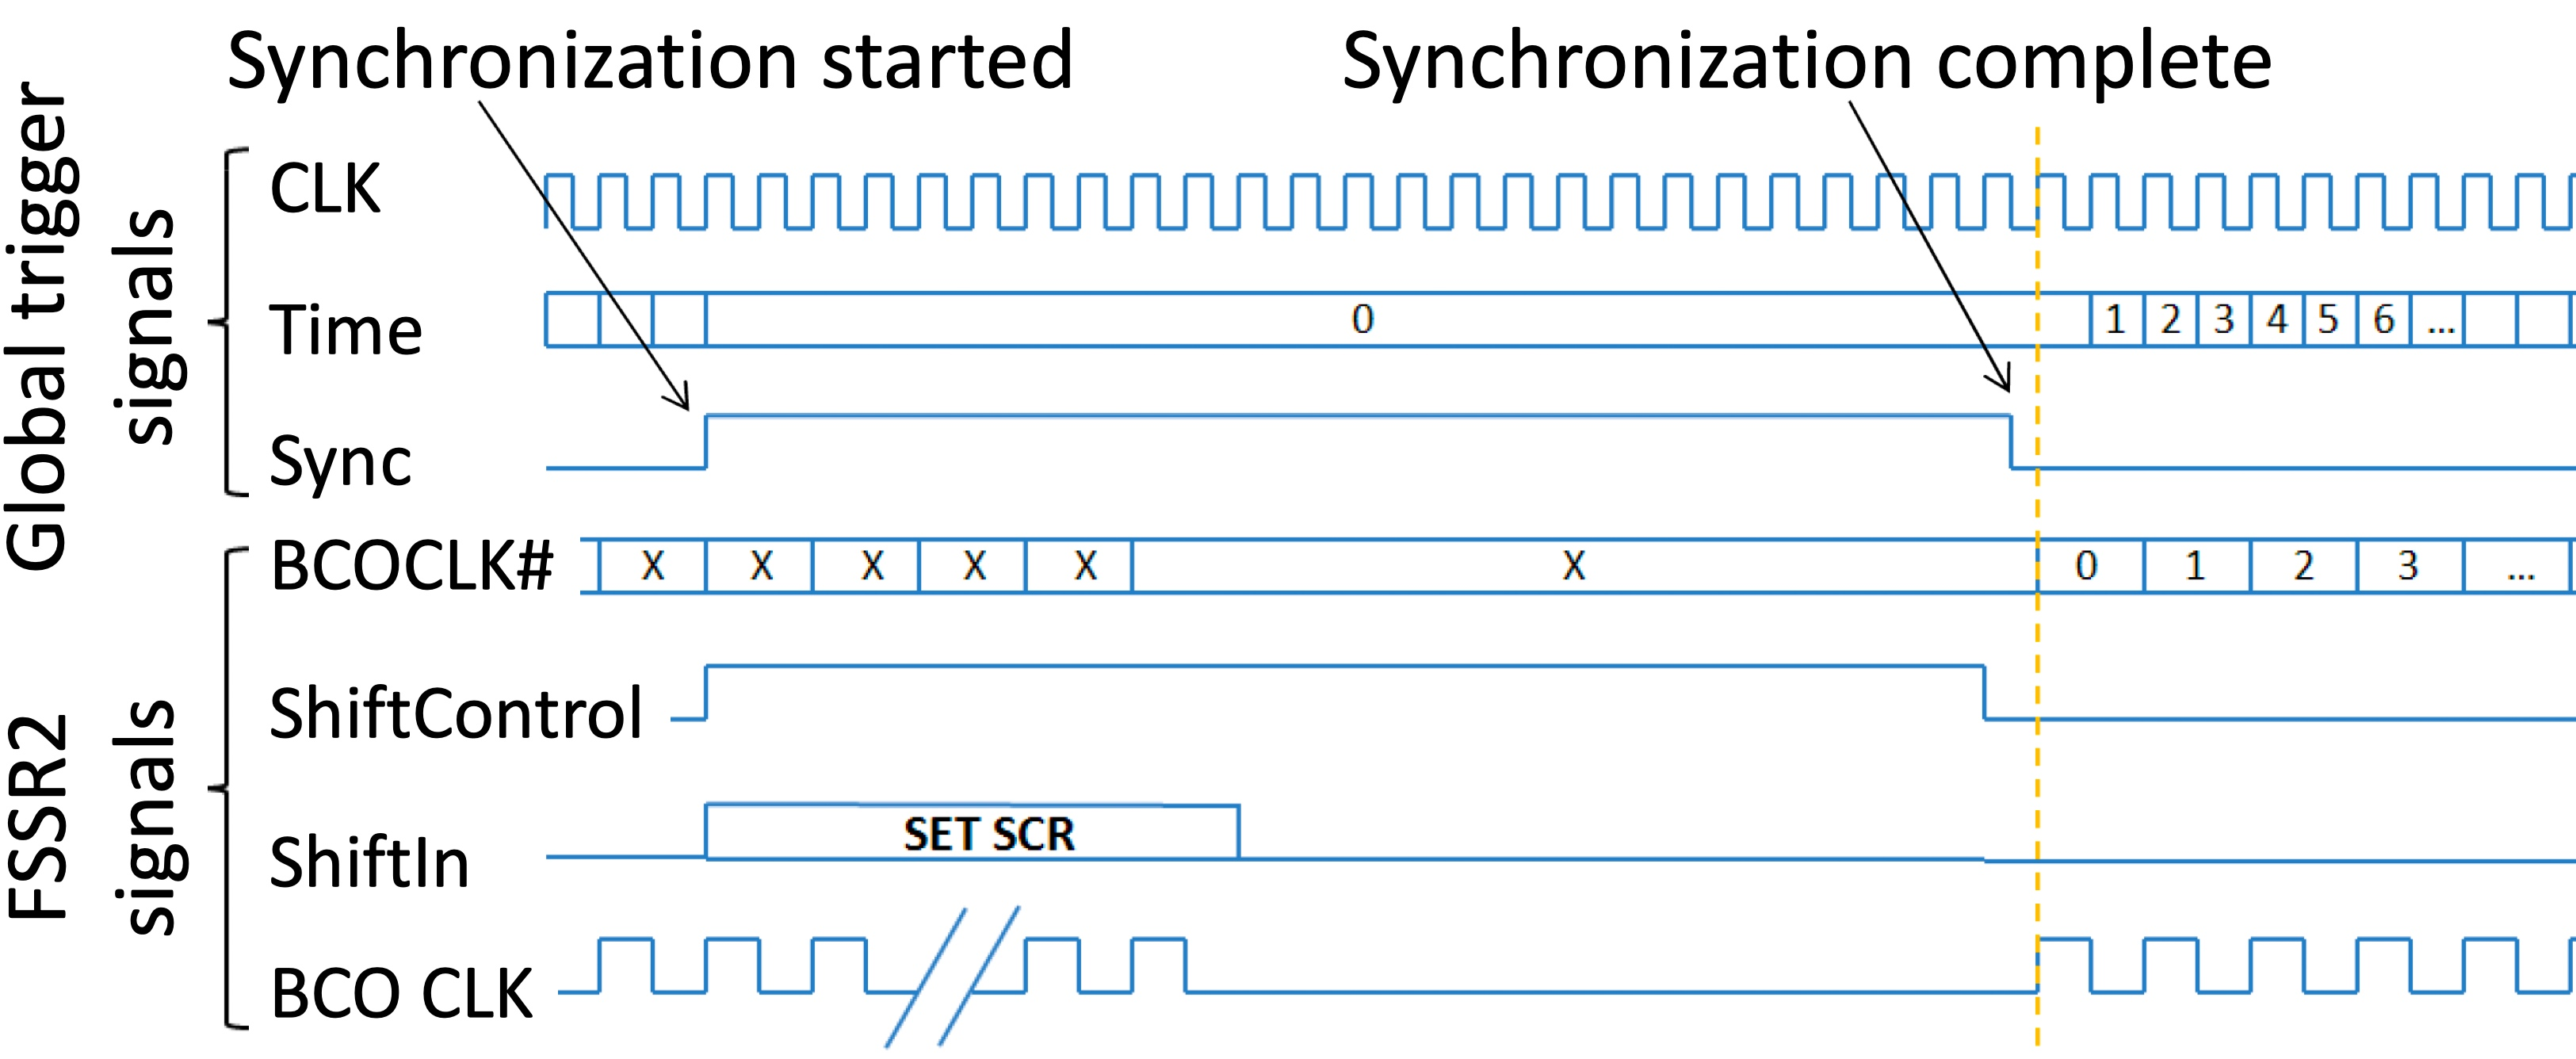
\includegraphics[width=1.0\columnwidth,keepaspectratio]{fssr2-sync.jpg}
\caption{FSSR2 clock and timestamp synchronization.}
\label{fig:fssr2-sync}
\end{figure}

\subsection{Back-End Readout}

The four FSSR2 ASICs on the HFCB communicate with the VXS architecture-based segment collector module (VSCM). The main purpose of the VSCM is to convert the FSSR2 data-driven information stream into the sparcified and triggered events that are correlated with external detectors. Idle status words are suppressed to minimize event size, but these status words are monitored for diagnostic purposes of the individual FSSR2 chips. The VSCM configures the FSSR2 ASIC registers, provides analog calibration pulses to the FSSR2 ASICs, sets/monitors proper control signals (clock, reset, status), and acquires serialized event data from the FSSR2 ASICs. Each VSCM can interface with two HFCBs. Up to 16 VSCM cards can reside in a VXS crate. When multiple VSCM cards are used, additional cards, the Trigger Interface (TI) and Signal Distribution (SD), are required to ensure event and timing synchronization. The VSCM supports a stand-alone mode, useful when only one or two HFCBs are used. The event builder of the VSCM uses the BCO clock timestamp from the data word of each FSSR2 ASIC and matches it to the timestamp of the global system clock, given by the CLAS12 trigger. Figure ~\ref{fig:fssr2-sync} shows the timing diagram for the FSSR2 clock and timestamp synchronization. The global trigger system "CLK" and "SYNC" signals are used by VSCM to phase align the BCO clocks  and counters across all FSSR2 chips. When SYNC is asserted, the BCO clock is halted after a smart reset is issued to the FSSR2. When SYNC is released, the BCO clock is started with its rising edge aligned to the global trigger clock rising edge. The FSSR2 ASIC data is tagged with a global trigger timestamp (48 bits, 8 ns resolution). Since the BCO clock is derived from the global system clock, triggers received by the VSCM will cause the event builder to extract only the hits with specific BCO timestamps that correspond to a programmable time window where the physics event could have occurred. When a trigger is received, the data words from the FSSR2 ASICs are copied to an event buffer and pushed into an event FIFO. These events can be read out in order with other modules in the system while event-level synchronization across all modules in the system is maintained. The VME interface provides for event readout, access to the configuration registers on the VSCM, bridges access to the registers of the FSSR2 ASICs, and provides an interface to the CPU. The 32-bit address space, 2 MB in size, is dedicated to the event builder FIFO, which can be read using single-cycle and block transfer VME protocols. Block transfer protocols are used for event readout; the 2eSST protocol used is to maximize performance. The 2eSST protocols provide ~200 MB/s sustained transfer rate and supports the proprietary JLab token-passing scheme that allows a single direct memory access (DMA) operation on the CPU to transfer data from all VSCM modules sequentially, eliminating overhead (compared to individual board transfers). The VSCM is set up to extract event data within a programmable lookback window of $\sim$16~$\mu$s relative to the received trigger. 

\begin{figure}[hbt] 
\centering 
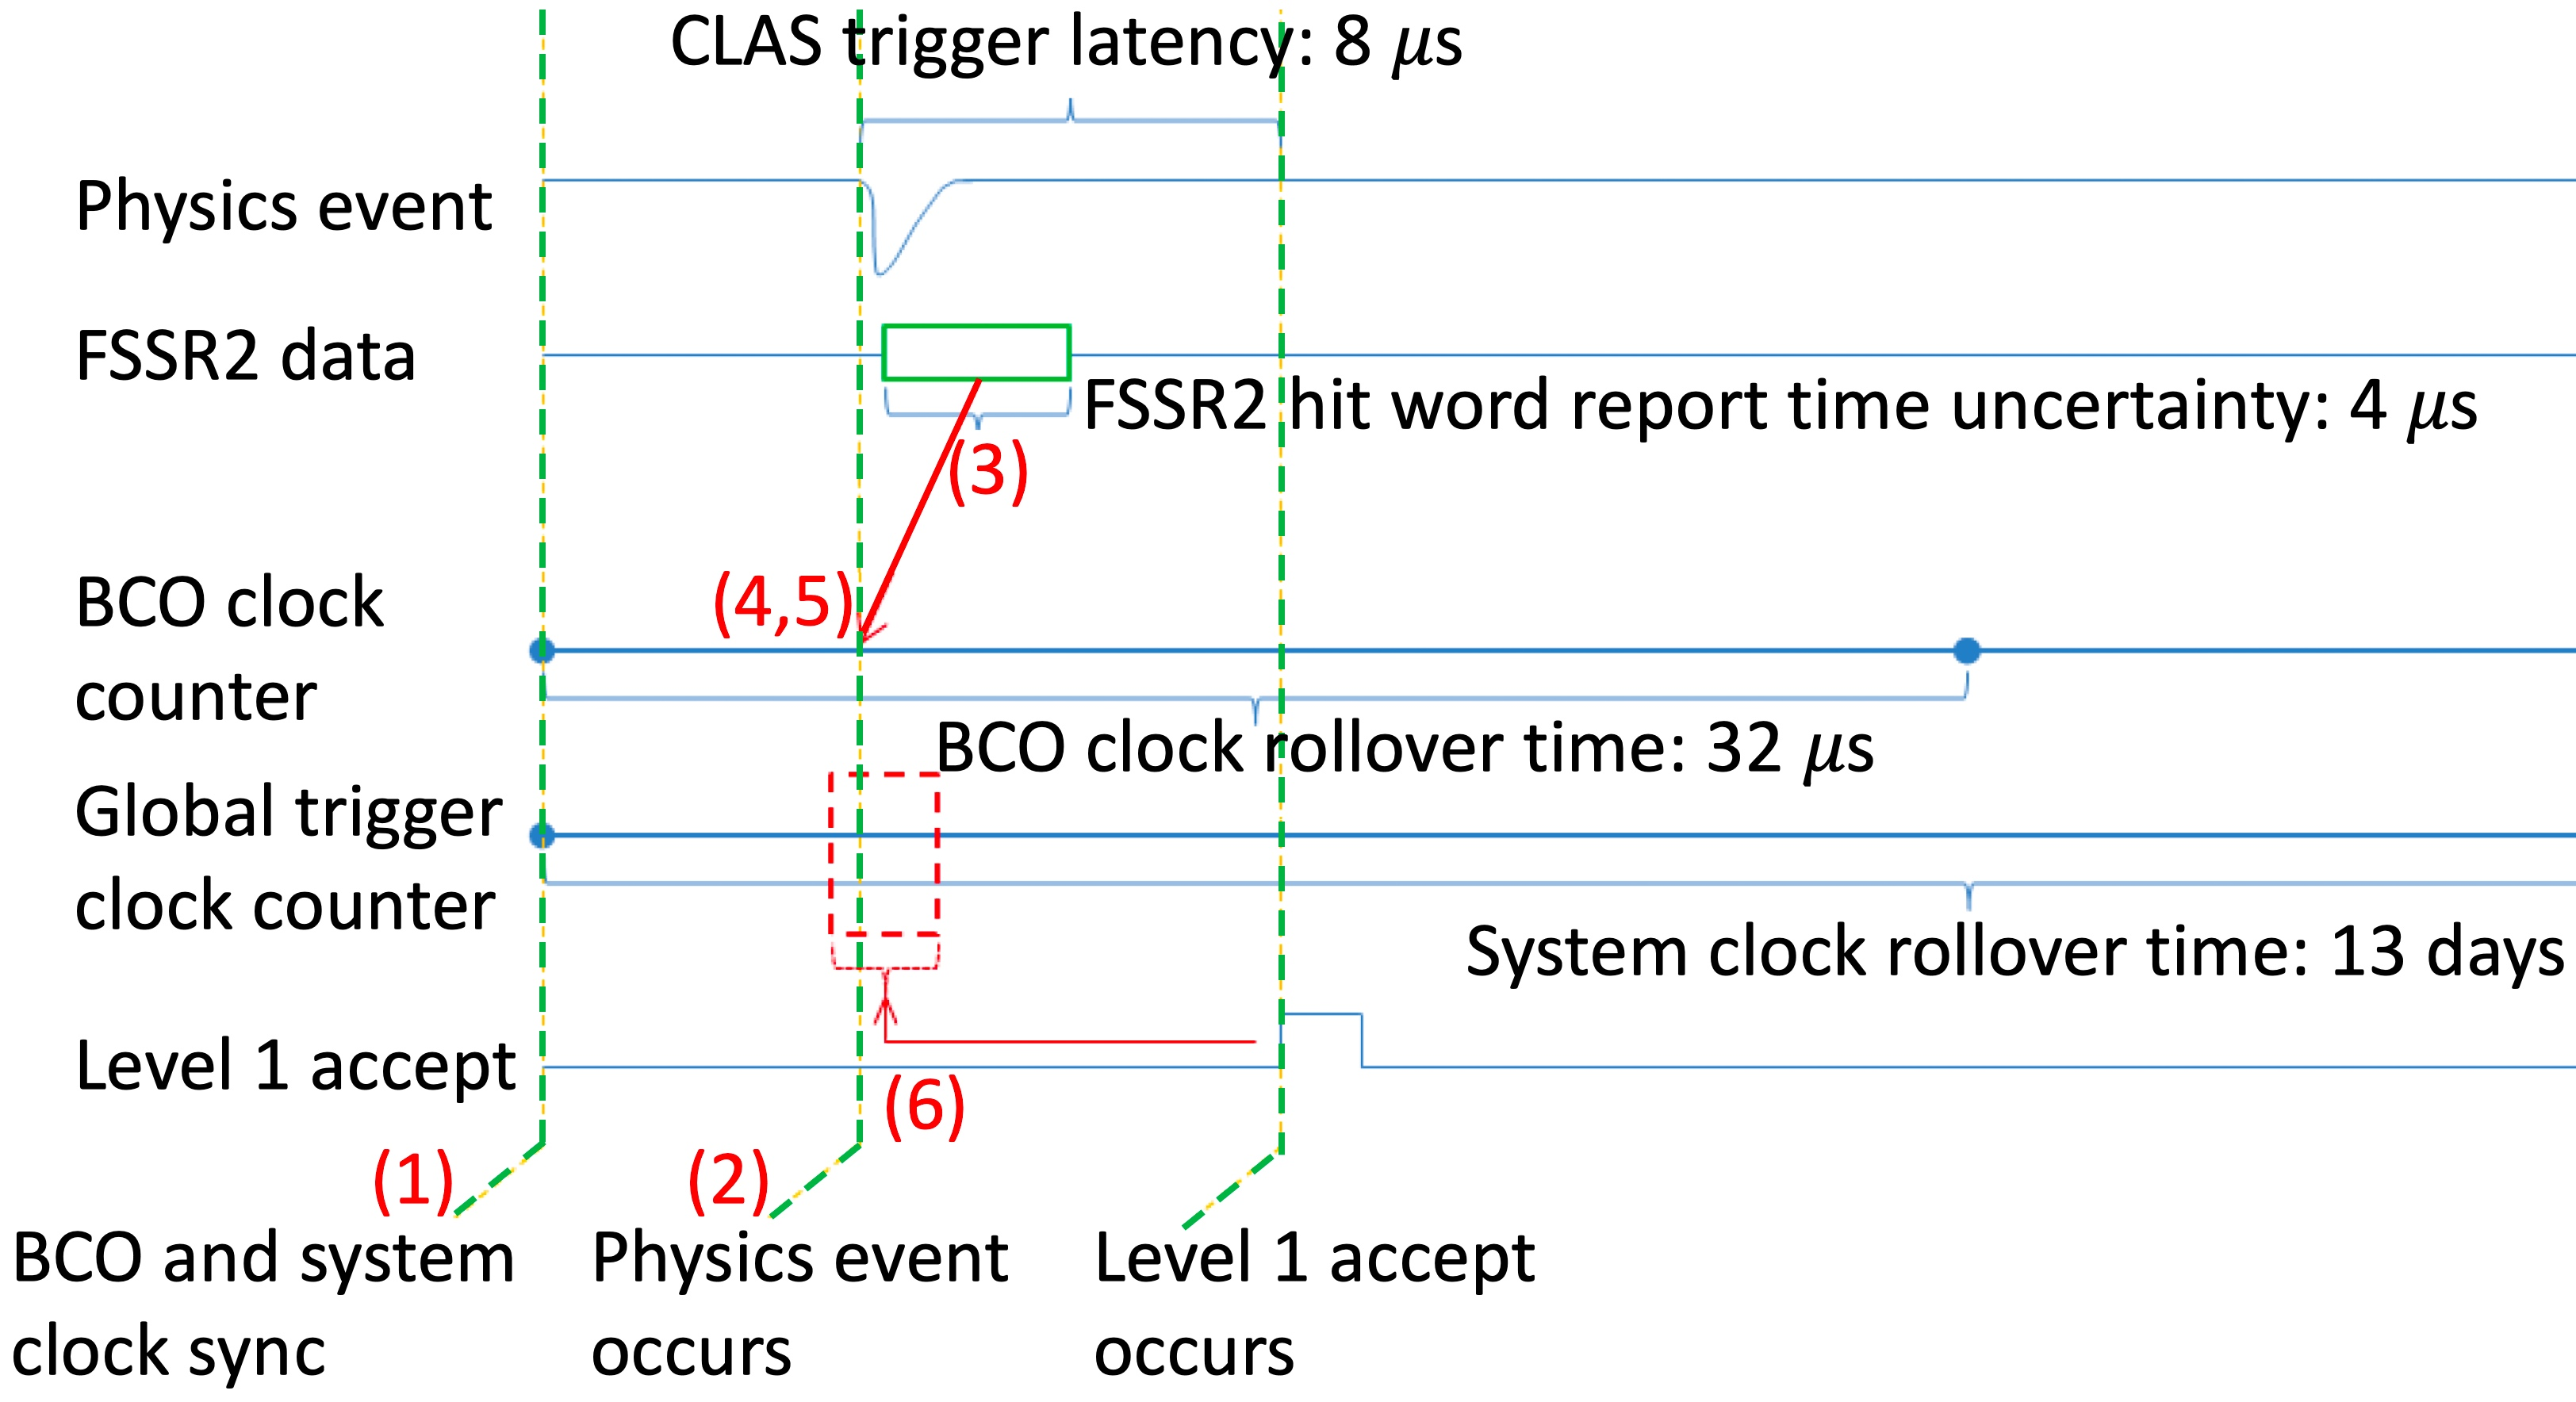
\includegraphics[width=1.0\columnwidth,keepaspectratio]{vscm-event-trigger.jpg}
\caption{VSCM event triggering.}
\label{fig:vscm-event-trigger}
\end{figure}

The VSCM design makes the FSSR2 data-driven architecture compatible with the CLAS12 free running DAQ. Figure~\ref{fig:vscm-event-trigger} describes the VSCM event triggering. At (1) a system reset and synchronization is performed. A physics event occurs at (2). At (3) the FSSR2 time unsorted hits arrive. At (4) the VSCM tags hits with the global trigger counter using the BCO number. The VSCM stores hits in the FIFO by the strip number at (5). At (6) level 1 accept received the FSSR2 hits with the global trigger counter matching the trigger window. The VSCM can handle large detector occupancies.

\begin{figure}[hbt] 
\centering 
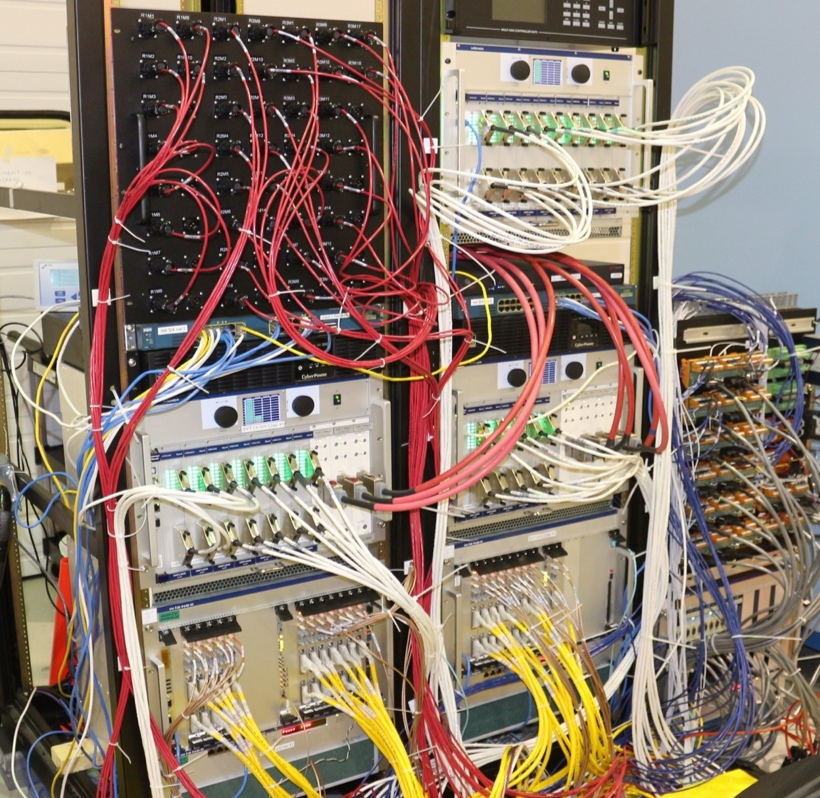
\includegraphics[width=1.0\columnwidth,keepaspectratio]{svt-test-stand.jpg}
\caption{The SVT test stand installed in the clean room.}
\label{fig:svt-test-stand}
\end{figure}

The calibration pulser circuit provides a 2 Vpp dynamic range, up to 125 MS/s, and 14-bit resolution (for pulse height steps in sub mV increments). The bandwidth is sufficient to allow 10 ns rise times to be delivered over 15 feet of 50~$\Omega$ coax cable terminated with 50~$\Omega$. Two independent pulser outputs are provided to drive both HFCB modules. The pulser signal phase can be placed in a deterministic phase relationship to the BCO clock that drives the FSSR2 ASIC. 

During the SVT integration and testing a full-featured test stand (see Fig. ~\ref{fig:svt-test-stand}) accommodating production services (power supplies, DAQ, slow controls, alarm handler, purging, and cooling system) for the whole detector was installed in the clean room.

\subsection{Expected Noise Performance}

The sensor thickness and total length of the strips (33 cm) are defined by the technical requirements on the detector acceptance and energy spectrum of the registered tracks. The signal generated in 320 $\mu$m sensors is about 24000 electrons which makes it essential to minimize all sources of noise and to control the cross-talk. 

\begin{figure}[hbt] 
\centering 
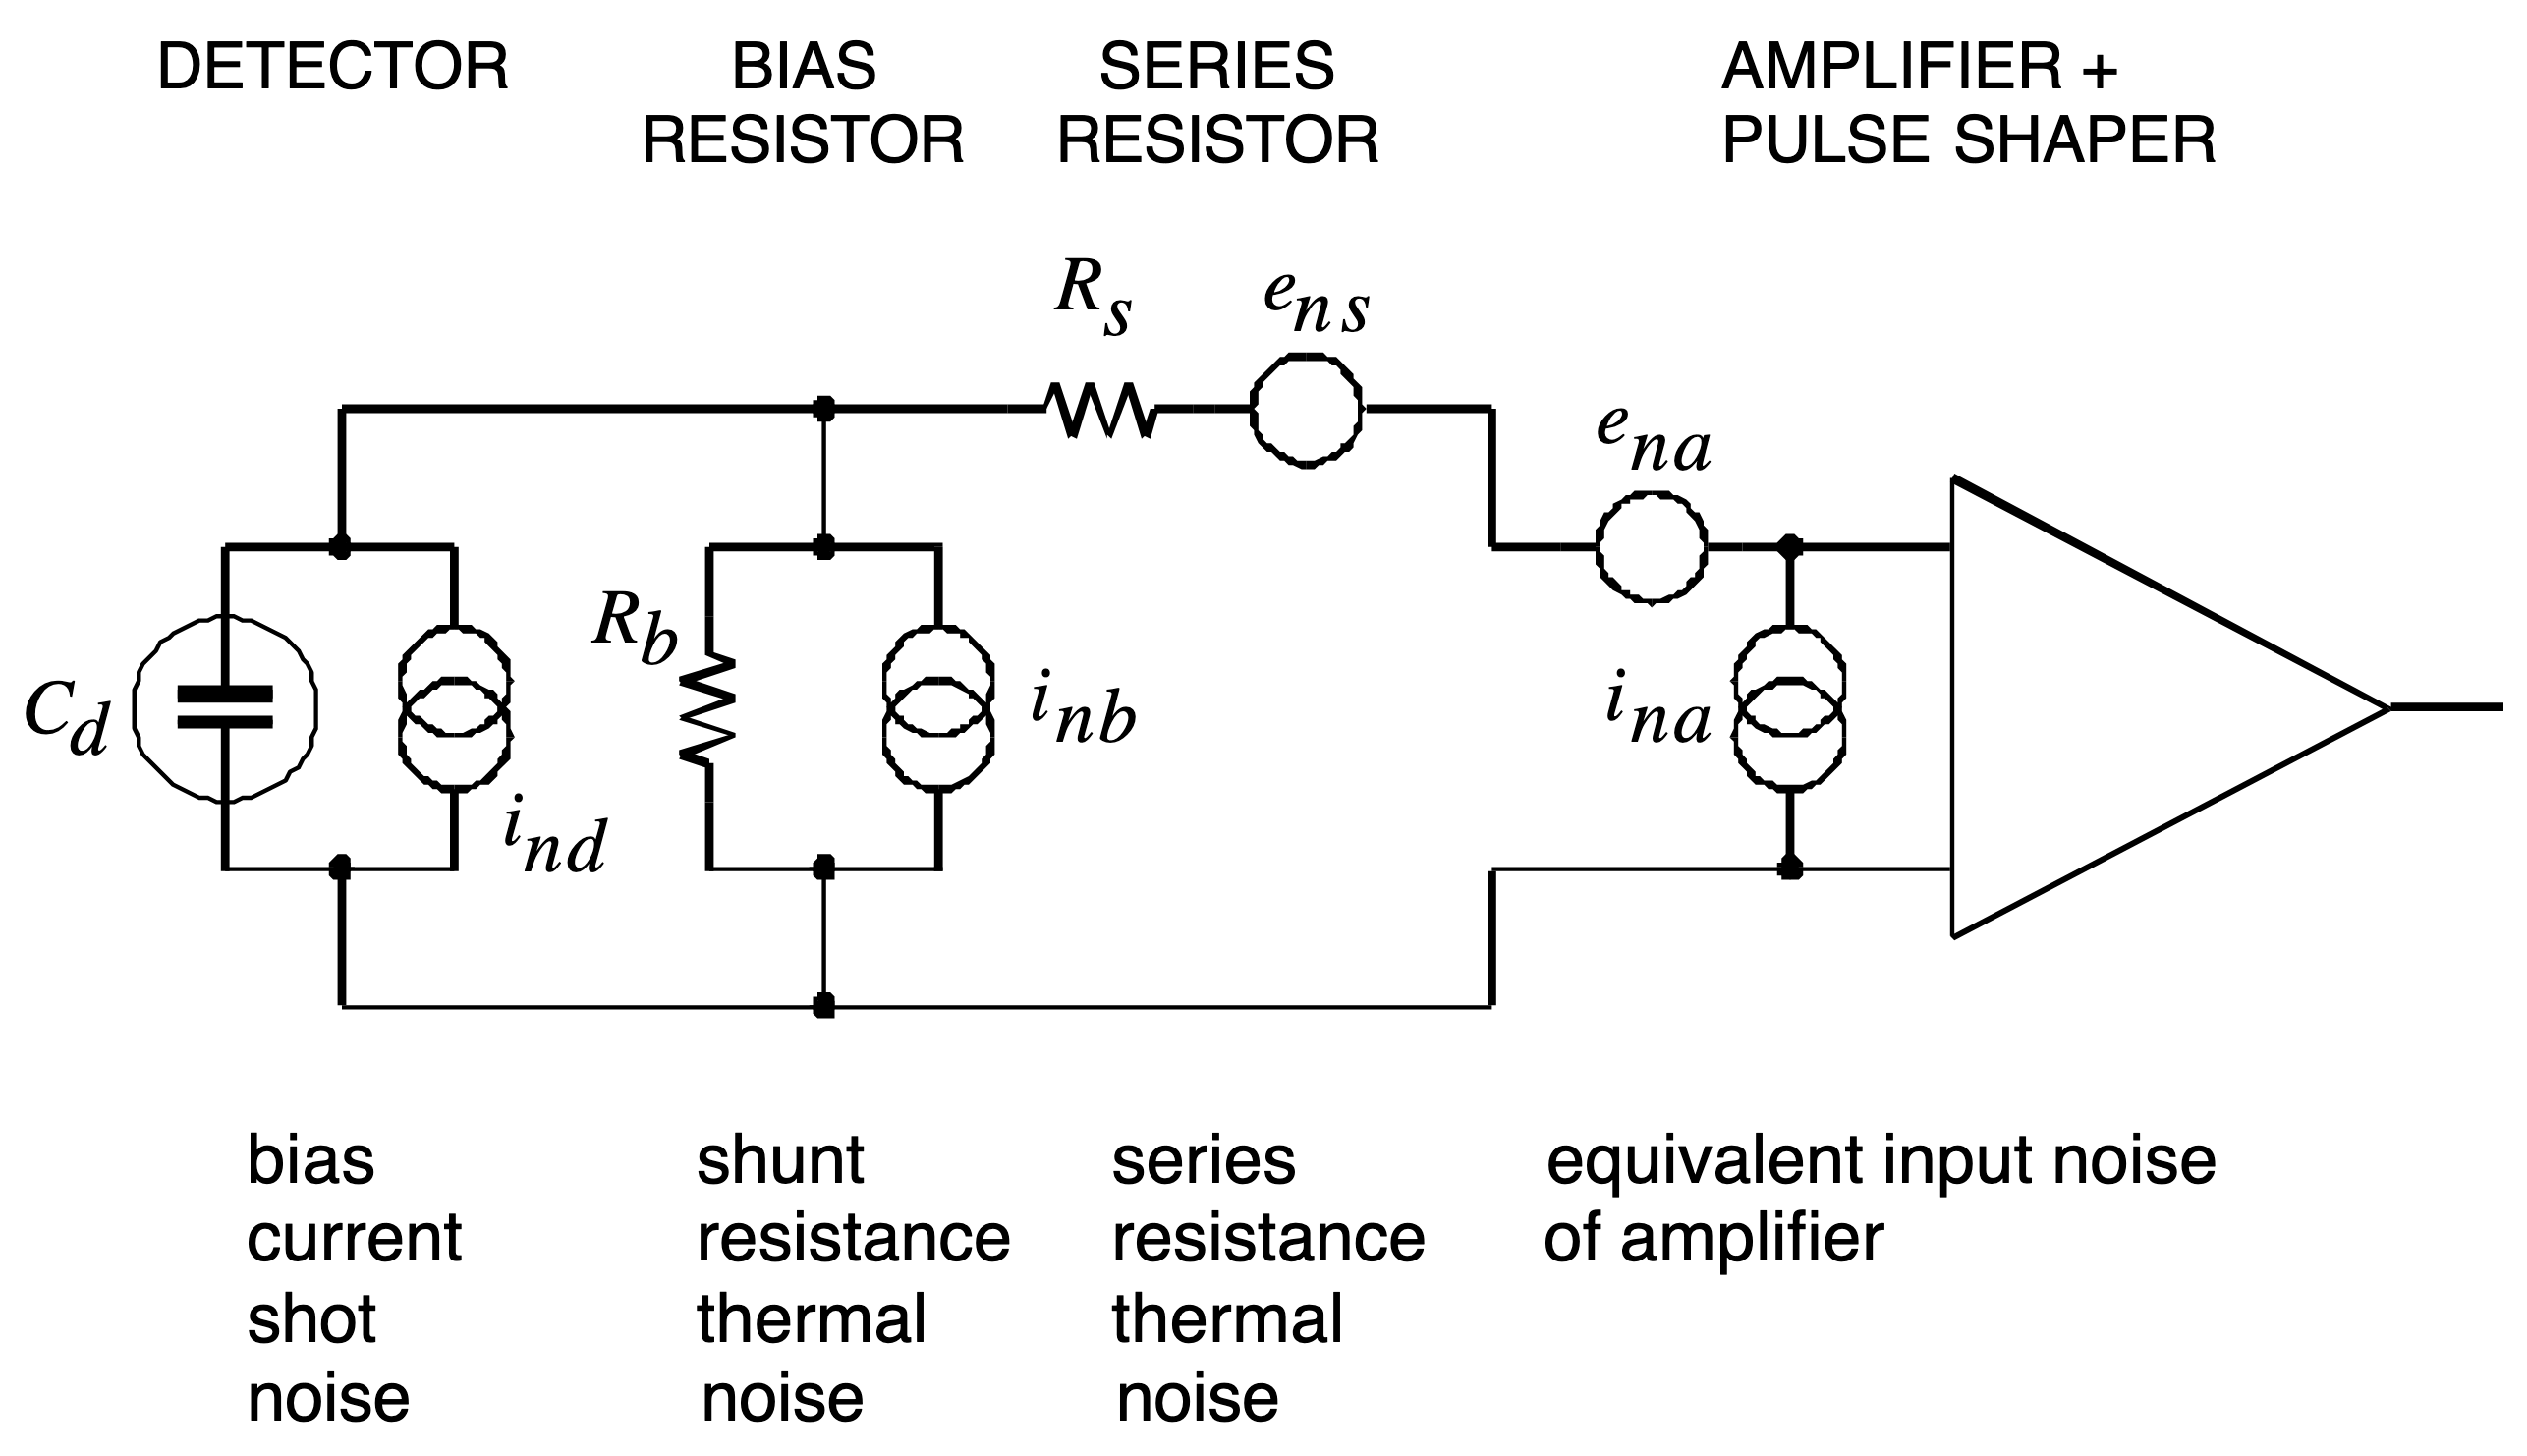
\includegraphics[width=1.0\columnwidth,keepaspectratio]{equivalent-noise-scheme.png}
\caption{Equivalent noise circuit diagram. Serial noise sources are shown as voltage sources and
parallel sources as current sources.}
\label{fig:equivalent-noise-scheme}
\end{figure}

The equivalent circuit diagram of a silicon strip sensor with connected readout electronics is shown in Fig.~\ref{fig:equivalent-noise-scheme}~\cite{SPIELER}. A single channel (3 daisy-chained strips) with capacitively coupled readout is represented by its total capacitance C$_{tot}$, a coupling capacitance C$_c$, the resistance of the connection line to the amplifier R$_s$, the bias resistor R$_b$ and a filtering capacitance of the bias circuit C$_b$. The SVT sensor measures the charge deposited by the particles, thus the noise is quoted in terms of the Equivalent Noise Charge (ENC), defined as the charge that, if injected in the input, gives a signal-to-noise ratio of 1. All the noise sources of a circuit can be summarized and represented by a noise voltage $v_{ni}$ appearing on the input of the amplifier. The internal capacitance of the amplifier $C_i$ is connected in parallel to $C_{tot}$. The dependence of the ENC $Q_n$ on the input capacitance can be parametrized as~\cite{BLOCHTHESIS}:

\begin{equation} Q^{RMS}_{n}=a+C_{tot}{\cdot}b  \label{eq:qn},
\end{equation}

where $a = v^{RMS}_{ni} \cdot (C_{f} + C_{i})$, $b = v^{RMS}_{ni}$, and $C_f$ is the feedback capacitance of the amplifier.

Parallel shot noise from the reverse bias current $I_b$ through the strip can be expressed as:

\begin{equation} \frac{1}{q_e}\frac{e}{\sqrt{8}}\sqrt{2q_eI_b\tau} \approx 108\cdot\sqrt{I_b[\mu A]\tau [ns]}  \label{eq:bias},
\end{equation}

where $q_e$ is charge of the charge carriers and $\tau$ is the characteristic shaping time.

Parallel noise from shunt resistance $R_b$ is:

\begin{equation} \frac{1}{q_e}\frac{e}{\sqrt{8}}\sqrt{\frac{4kT}{R_b\tau}} \approx A\cdot\sqrt{\frac{\tau [ns]}{R_b[M \Omega]}} \label{eq:shunt},
\end{equation}

where $k$ is the Boltzmann constant and $T$ is the temperature, $A$ is the temperature dependent factor equal to 24 at 20$\degree$C and 22.5 at -10$\degree$C.

Series noise from metal strip resistance $R_s$ is:

\begin{equation} \frac{1}{q_e}\frac{e}{\sqrt{8}}\sqrt{4kT\frac{R_s}{3\tau}C_{tot}} \approx B\cdot C_{tot}[pF]\cdot\sqrt{\frac{R_s[\Omega]}{\tau [ns]}} \label{eq:strip},
\end{equation}

where $B$ is the temperature dependent factor equal to 14 at 20$\degree$C and 13 at -10$\degree$C.

For non-irradiated sensors the shot noise from the measured sensor reverse bias current 0.05--0.4 $\mu$A (256 strips) at -10--20$\degree$C is within 20-50 electrons with a shaping time of 125 ns and can be neglected. As demonstrated in Eqs. (\ref{eq:shunt}) and (\ref{eq:strip}), the detector noise does not change much when the sensors are cooled up to -10$\degree$C. The contribution from the shunt resistance is about 200 electrons with a shaping time of 125 ns. The total capacitance of the strip $C_{tot}$ including the wire bonds and the pitch adapter is $\sim$45 pF. The metal strip (33 cm) resistance is $\sim$230 $\Omega$, which gives an estimate for the series noise of $\sim$850 electrons.

Figure~\ref{fig:fssr2-enc-c} shows the results of the FSSR2 noise measurements performed on a single-chip test board with discrete capacitors connected to the amplifier confirming linear dependence of the noise on the total capacitive load of the amplifier in Eq. (\ref{eq:qn}). The contribution from the amplifier itself is the dominant source of noise, mainly caused by shot noise and thermal noise on the current path of the transistors. Adding all sources of noise gives an estimate for the total ENC for the SVT channel $\sim$1500--1600 electrons.

\begin{figure}[hbt] 
\centering 
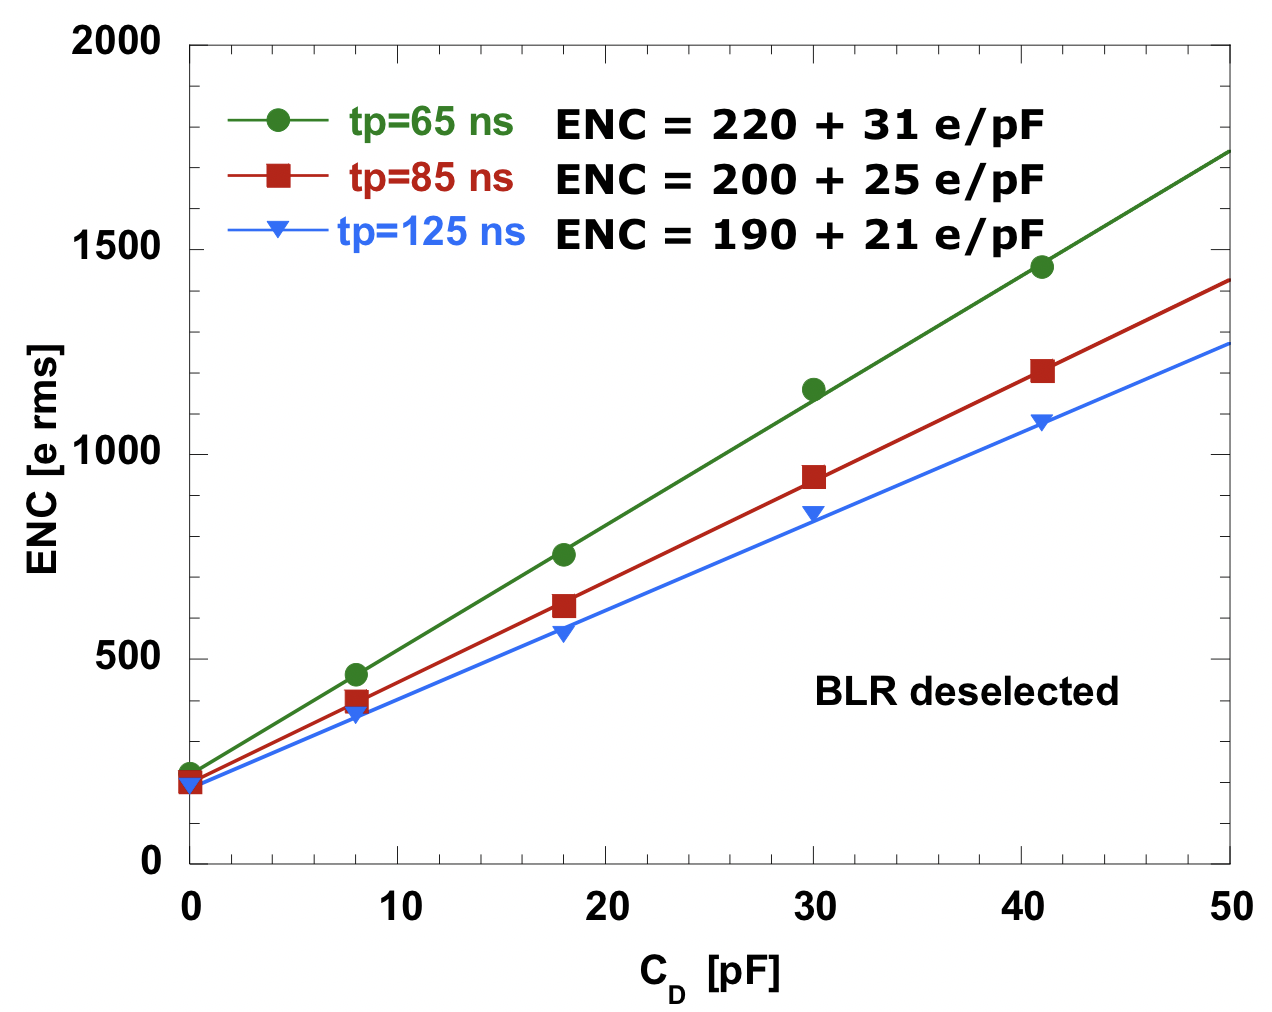
\includegraphics[width=1.0\columnwidth,keepaspectratio]{fssr2-enc-c.png}
\caption{FSSR2 ENC vs. detector capacitance at different shaping time settings.}
\label{fig:fssr2-enc-c}
\end{figure}
